\documentclass[a4paper,12pt]{article}        
\usepackage{geometry}           % пакет для задания полей страницы командой \geometry
\geometry{left=3cm,right=1.5cm,top=2cm,bottom=2cm}
% \usepackage[cp1251]{inputenc}   % кодировка текста
\usepackage{mathtext}           % позволяет использовать русские буквы в формулах
\usepackage[T2A]{fontenc}       %пакет Т2А необходим для правильного отображения кириллицы и переноса слов
%\inputencoding{cp1251}          % тоже кодировка...
\usepackage[russian]{babel}     % языковой пакет - последний язык главный
%\usepackage[unicode]{hyperref}  %создаёт гиперссылки на список литературы в pdf-файле
\usepackage{amstext,amsmath,amssymb}            % пакеты для формул
\usepackage{bm}                 % boldmath - пакет для жирного шрифта
\usepackage[pdftex]{graphicx}   % пакет для включения рисунков в форматах png,pdf,jpg,mps,tif
                                % надо компилировать сразу в pdf
\usepackage{amsfonts}           % греческие символы и, возможно, что-то ещё
\usepackage{indentfirst}        % одинаковый отступ для первого параграфа и всего остального
\usepackage{cite}               % команда /cite{1,2,7,9} даёт ссылки
\usepackage{multirow}           % пакет для объединения строк в таблице: надо указать число строк и ширину столбца
\usepackage{array}              % нужен для создания таблиц
\linespread{1.3}                % полтора интервала. Если 1.6, то два интервала
\pagestyle{plain}               % номерует страницы

% \documentclass[a4paper,12pt]{article} 
\usepackage{geometry}           % пакет для задания полей страницы командой \geometry
\geometry{left=3cm,right=1.5cm,top=2cm,bottom=2cm}
% \usepackage[cp1251]{inputenc}   % кодировка текста
\usepackage{mathtext}           % позволяет использовать русские буквы в формулах
\usepackage[T2A]{fontenc}       %пакет Т2А необходим для правильного отображения кириллицы и переноса слов
%\inputencoding{cp1251}          % тоже кодировка...
\usepackage[russian]{babel}     % языковой пакет - последний язык главный
%\usepackage[unicode]{hyperref}  %создаёт гиперссылки на список литературы в pdf-файле
\usepackage{amstext,amsmath,amssymb}            % пакеты для формул
\usepackage{bm}                 % boldmath - пакет для жирного шрифта
\usepackage[pdftex]{graphicx}   % пакет для включения рисунков в форматах png,pdf,jpg,mps,tif
                                % надо компилировать сразу в pdf
\usepackage{amsfonts}           % греческие символы и, возможно, что-то ещё
\usepackage{indentfirst}        % одинаковый отступ для первого параграфа и всего остального
\usepackage{cite}               % команда /cite{1,2,7,9} даёт ссылки
\usepackage{multirow}           % пакет для объединения строк в таблице: надо указать число строк и ширину столбца
\usepackage{array}              % нужен для создания таблиц

\usepackage{titlesec}
\usepackage{enumitem}

\usepackage{graphicx}
   
\usepackage{subcaption}   

\titleformat{\section}[block]{\centering\bfseries\huge}{Глава \thesection.}{1em}{}
\usepackage{caption}
\renewcommand{\thefigure}{\thesubsection.\arabic{figure}}
\DeclareCaptionLabelSeparator{bar}{\space--\space}
\captionsetup{labelsep=bar,justification=centering}

\linespread{1.3}                % полтора интервала. Если 1.6, то два интервала
\pagestyle{plain}               % номерует страницы


\begin{document}
\begin{titlepage}
\begin{center}
БЕЛОРУССКИЙ ГОСУДАРСТВЕННЫЙ УНИВЕРСИТЕТ

ФИЗИЧЕСКИЙ ФАКУЛЬТЕТ

Кафедра компьютерного моделирования физических процессов
\end{center}

\vspace{5cm}

\begin{center}
\LARGE {ДИПЛОМНАЯ РАБОТА}
\end{center}

\begin{center}
\LARGE \bf{Компьютерное моделирование случайно распределенных ансамблей частиц для задач континуальной перколяции}
\end{center}

\vspace{2cm}

\large
\begin{flushright}
\textbf{Выполнил:}\\
студент V курса \\
Запорожцев Александр Викторович\\

\vspace{0.5cm}

\textbf{Научный руководитель:}\\
кандидат физико-математических наук, \\
старший преподаватель Федотов Александр Сергеевич
\end{flushright}
\vspace{0.5cm}

\begin{flushright}
\textbf{Рецензент:}\\
Надеюсь кто-нибудь будет :) 
\end{flushright}

\vspace{1cm}

\begin{center}
Минск 

2021
\end{center}

\end{titlepage}


\begin{center}
\LARGE\bf{Аннотация}
\end{center}

Текст аннотации

\setcounter{page}{2}            % Нумерация страинц начинается с "2"

\newpage                        % Начинает текст с новой страницы
\tableofcontents                % Автоматическое создание оглавления по названиям разделов, подразделов и т.п.

\newpage

% \begin{center}
\LARGE\bf{Введение}
\end{center}


\newpage

\section{New section}

\section{Глава 1. Современные подходы к генерации ансамблей}

Текст раздела.

................................................

\begin{equation}
 \begin{aligned}
  \mathbf E^h=\pm i\mathbf H^e,\quad\mathbf H^h=\mp i\mathbf E^e. % Пример жирного шрифта
 \end{aligned}
\end{equation}

.................................................

\begin{equation}            % Пример большой формулы, где нужно переносить часть выражения на другую строчку
 \label{Eeexplicit}         % Когда нужны большие скобки, их можно открывать и закрывать с помощью \left( и \right(
 \begin{aligned}            % для случая круглых скобок. Когда надо открыть скобку на одной строке, а закрыть на другой,
  \mathbf E^e=\frac{E_0e^{-i\varphi}}{(1+2i\chi)^2}\exp\left(-\frac{\xi^2}      % надо в конце первой сроки поставить \right.,
  {1+2i\chi}\right)\left\{\left(1-\frac{\xi^2}{1+2i\chi}\right)\mathbf          % а в начале следующей - \left.
  e_x+\right.\\
  \left.+\frac{\xi^2}{1+2i\chi}(\cos2\phi\,\mathbf e_x+\sin2\phi\,\mathbf e_y)\right\}
 \end{aligned}
\end{equation}
\begin{equation}
 \label{Heexplicit}
 \begin{aligned}
  \mathbf H^e=\frac{E_0e^{-i\varphi}}{(1+2i\chi)^2}\exp\left(-\frac{\xi^2}
  {1+2i\chi}\right)\left\{\left[1-\frac{\xi^2}{1+2i\chi}-\right.\right.\\
  \left.-\frac{2\Delta^2}{1+2i\chi}\left(2-\frac{4\xi^2}
  {1+2i\chi}+\frac{\xi^4}{(1+2i\chi)^2}\right)\right]\mathbf e_y-\\
  -\frac{\xi^2}{1+2i\chi}\left[1-\frac{2\Delta^2}{1+2i\chi}\left(3-\frac{\xi^2}{1+2i\chi}\right)\right]
  (\sin2\phi\,\mathbf e_x-\cos2\phi\,\mathbf e_y)-\\
  \left.-\frac{4i\Delta\xi}{1+2i\chi}
  \left(2-\frac{\xi^2}{1+2i\chi}\right)\sin\phi\,\mathbf e_z\right\}
 \end{aligned}
\end{equation}

\begin{figure}[pH]                          % Пример рисунка, состоящего из 6 картинок
\begin{minipage}[h]{0.47\linewidth}         % Создаём "маленькие" рисунки шириной 47% от ширины страницы
\center{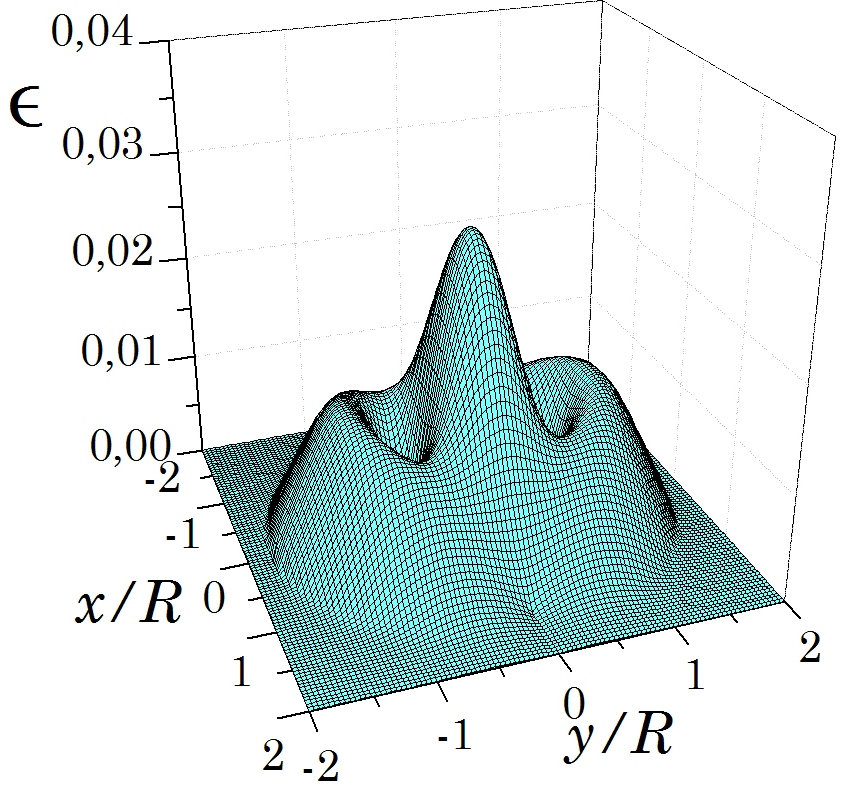
\includegraphics[width=1.0\linewidth]{images/EGraph1}} % Вставляем рисунок в полученное "окно" полностью - 100%
\end{minipage}
\hfill                                      % Следующий рисунок правее
\begin{minipage}[h]{0.47\linewidth}
\center{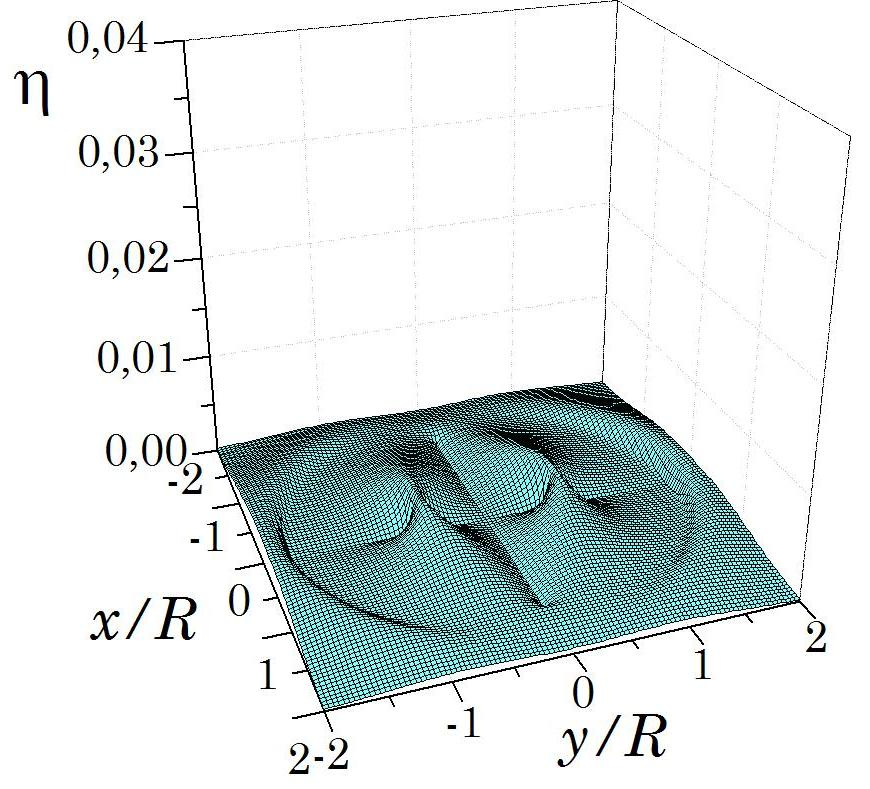
\includegraphics[width=1.0\linewidth]{images/HGraph1}}
\end{minipage}
\vfill                                      % следующий рисунок ниже - слева
\begin{minipage}[h]{0.47\linewidth}
\center{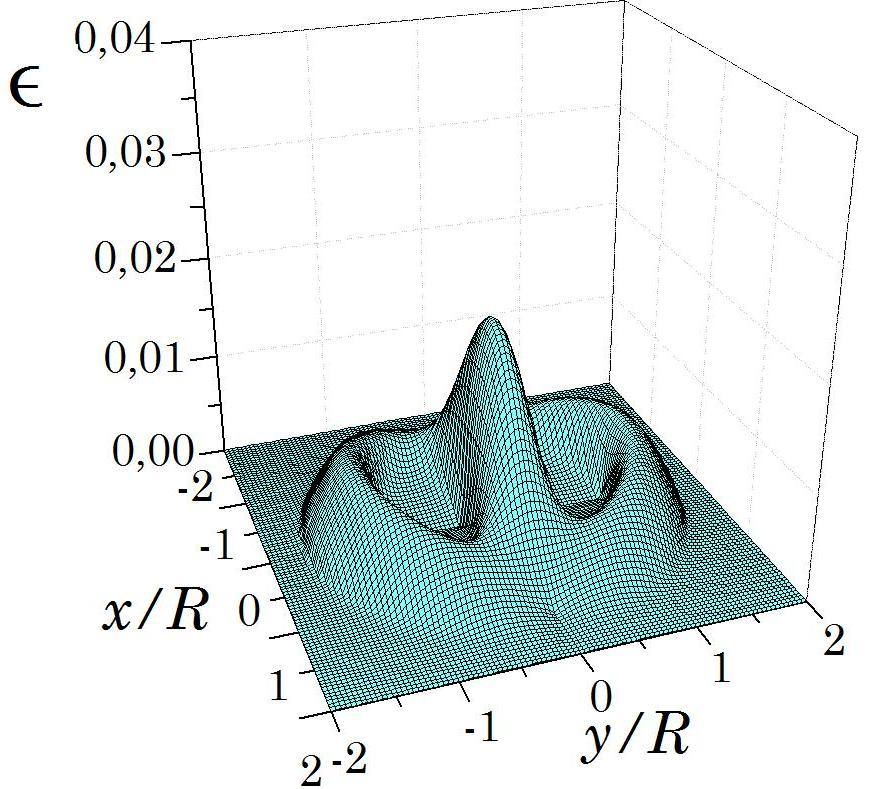
\includegraphics[width=1.0\linewidth]{images/EGraph2}}
\end{minipage}
\hfill
\begin{minipage}[h]{0.47\linewidth}
\center{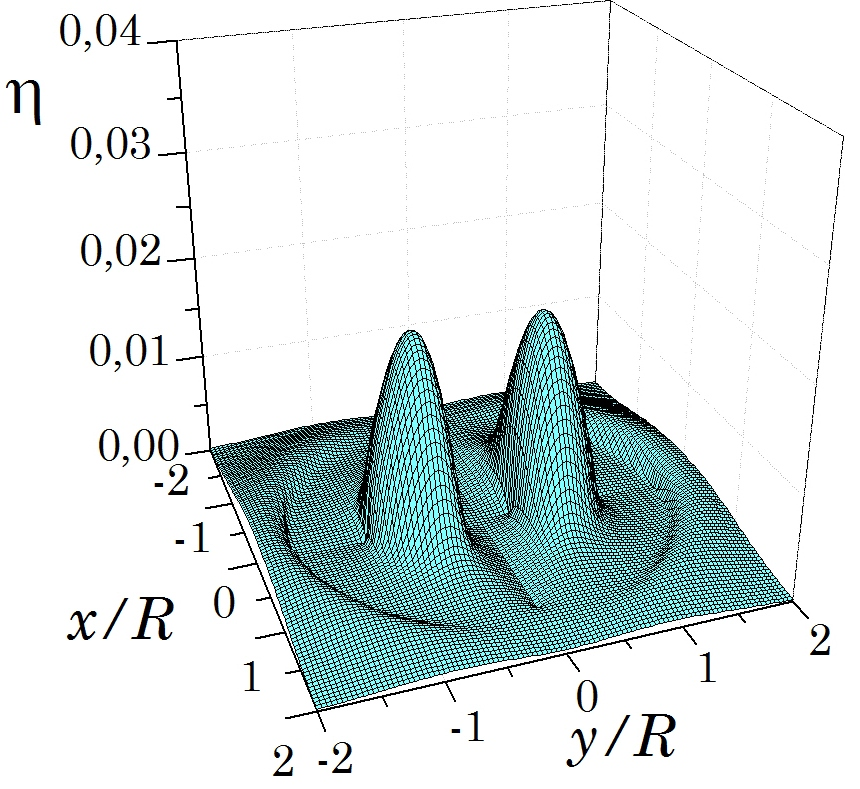
\includegraphics[width=1.0\linewidth]{images/HGraph2}}
\end{minipage}
\vfill
\begin{minipage}[h]{0.47\linewidth}
\center{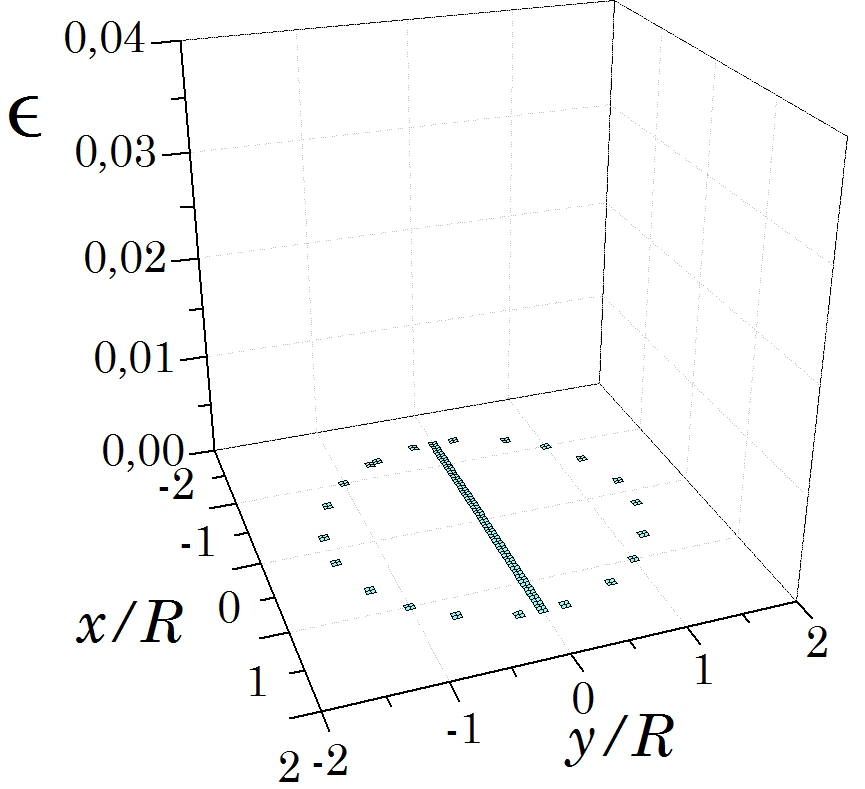
\includegraphics[width=1.0\linewidth]{images/EGraph3}}
\end{minipage}
\hfill
\begin{minipage}[h]{0.47\linewidth}
\center{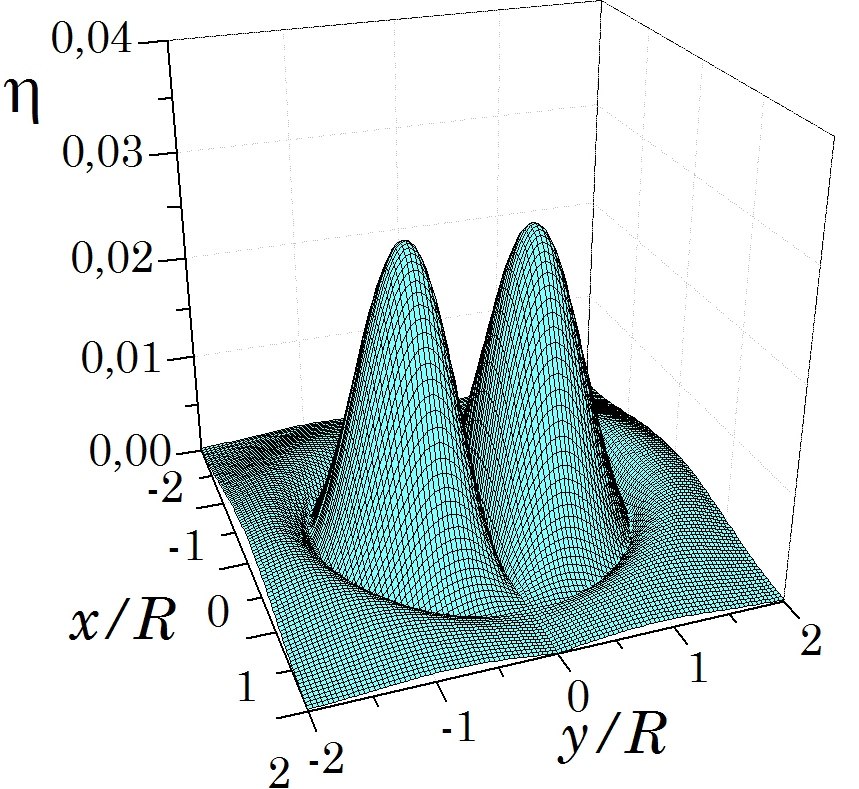
\includegraphics[width=1.0\linewidth]{images/HGraph3}}
\end{minipage}
\caption{\footnotesize Инварианты $\epsilon$ и $\eta$ для случая
одиночного линейно-поляризованного импульса $e$-типа в моменты
времени $t=0$, $t=\pi/4\omega$, $t=\pi/2\omega$. Остальные параметры
положены равными $E_0=0.1$, $z=0$, $\Delta=0.1$.} \label{EHinvs}   % Лейбл для ссылки на рисунок с помощью "рис.~\ref{EHinvs}"
\end{figure}

На рис.~\ref{EHinvs} показаны зависимости инвариантов $\epsilon$ и
$\eta$ от пространственных координат $x$ и $y$ в плоскости $z=0$ в
моменты времени $t=0$, $t=\pi/4\omega$, $t=\pi/2\omega$.


\newpage


\section{Раздел 2}

Текст раздела


\subsection{Подраздел 1}

        % Пример таблицы. \multirow{x}{Ycm} позволяет объединить x строк в столбце, длину которого задаём равной Y см

\begin{table}[t]
\caption{\label{table1}Среднее число пар, рождённых одиночным
(слева) и двумя сталкивающимися (справа) циркулярно-поляризованными
импульсами $e$-типа из вакуума, $\Delta=0.1$}
\begin{center}
\begin{tabular}{|c|c|c|c|c|c|}
\hline \multirow{2}{2cm}{$I\cdot10^{-28}$,
Вт/см$^2$}&\multirow{2}{2cm}{\quad$E_0/E_S$}&
\multirow{2}{2.5cm}{$\qquad\,
N$}&\multirow{2}{2.5cm}{$I\cdot10^{-26}$, Вт/см$^2$}&
\multirow{2}{2.5cm}{\quad$E_0/E_S$}&\multirow{2}{2.5cm}{$\qquad\, N$}\\
&&&&&\\
\hline   0.6   &  0.203 &    1.94(-5) &1.0     &0.0262   & 2.36(-8)\\
\hline   0.8   &  0.234 &    5.57(-2) &1.5     &0.0321   & 3.12(-3)\\
\hline   1.0   &  0.262 &       13.4  &2.0     &0.0371   &    3.85\\
\hline   1.5   &  0.321 &     7.57(4) &2.5     &0.0414   &  5.20(2)\\
\hline   2.0   &  0.371 &     1.42(7) &3.0     &0.0454   &  2.01(4)\\
\hline   2.5   &  0.414 &     5.29(8) &4.0     &0.0524   &  3.59(6)\\
\hline   3.0   &  0.454 &     7.89(9) &5.0     &0.0586   &  1.33(8)\\
\hline   4.0   &  0.524 &    3.70(11) &6.0     &0.0642   &  1.95(9)\\
\hline   5.0   &  0.586 &    5.35(12) &7.0     &0.0693   & 1.61(10)\\
\hline   6.0   &  0.642 &    4.05(13) &8.0     &0.0741   & 8.94(10)\\
\hline   8.0   &  0.741 &    7.17(14) &9.0     &0.0786   & 3.75(11)\\
\hline  10.0   &  0.829 &    5.33(15) &10.0    &0.0829   & 1.28(12)\\
\hline
\end{tabular}
\end{center}
\end{table}

\subsection{Подраздел 2}

Текст подраздела

\newpage

\begin{center}
\LARGE\bf{Заключение}
\end{center}

\newpage

\begin{thebibliography}{99}
\addcontentsline{toc}{section}{Список использованной литературы}

\bibitem{menshikov}
М. В. Меньшиков, С. А. Молчанов, А. Ф. Сидоренко. \emph{Теория перколяции и некоторые приложения, Итоги науки и техн}, т. XXIV, Сер. Теор. вероятн. Мат. стат. Теор. кибернет.,   \textbf{53-57}, 110 (1986).


\bibitem{buzmakova}
М. M. Бузмакова. \emph{Перколяция сфер в континууме}, т. XII. Сер. Математика. Механика. Информатика, \textbf{48-55}, 49 (2012).

\bibitem{tarasevich}
Ю. Ю. Тарасевич. \emph{Перколяция: теория, приложения, алгоритмы}. Едиториал УРСС, \textbf{112} (2002). 

\bibitem{schlovsky}
Б. И. Шкловский, А. Л. Эфрос \emph{Электронные свойства легированных полупроводников}. Наука, \textbf{416} (1979). 

\bibitem{abrikosov}
A. A. Abrikosov, \emph{Spin glasses with short range interaction}.  т. 29. Adv. Phys. \textbf{869-946} (1980). 

\bibitem{mersen}
M. Malsumoto, \emph{Mersenne twister: A 623-dimensionally equidistributed uniform pseudorandom number generator}. ACM Trans, on Modeling and Computer Simulations.т. 8. \textbf{3-30} (1998). 

\bibitem{hoshen}
J. Hoshen, R. Kopelman. \emph{Percolation and cluster distribution. I. Cluster multiple labeling technique and critical concentration algorithm}. 11 Physical Review. т. 14,
№ 8. \textbf{3438-3445} (1976). 



\end{thebibliography}


\end{document}
